\documentclass[12pt]{article}
\usepackage{verbatim}
\usepackage[dvips]{epsfig}
\usepackage{color}
\usepackage{url}
\usepackage[colorlinks=true]{hyperref}

\begin{document}

\section*{GENESIS: Documentation}

{\bf Related Documentation:}
% start: userdocs-tag-replace-items related-do-nothing
% end: userdocs-tag-replace-items related-do-nothing

\section*{De Schutter: Purkinje Cell Model}

\subsection*{Source}

De Schutter E \& Bower JM (1994) An active membrane model of the cerebellar Purkinje cell I. Simulation of current clamp in slice. {\it Journal of Nerurophysiology}. {\bf 71}: 375--400. \\

\subsection*{Figure}

\begin{figure}[h]
\centering
   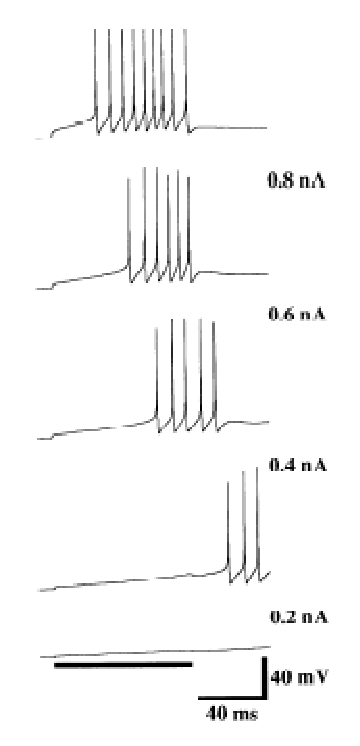
\includegraphics[scale=0.75]{figures/Fig.1.5.eps}
   \caption{Simulation of short current steps just below and above firing threshold in the soma (model PM9). Amplitude of current injection for each trace is indicated. Bar below traces: duration.}
   \label{fig:DS1.5}
\end{figure}


\end{document}
